% Created 2020-06-15 Mon 10:40
% Intended LaTeX compiler: pdflatex
\documentclass[presentation]{beamer}
\usepackage[utf8]{inputenc}
\usepackage[T1]{fontenc}
\usepackage{graphicx}
\usepackage{grffile}
\usepackage{longtable}
\usepackage{wrapfig}
\usepackage{rotating}
\usepackage[normalem]{ulem}
\usepackage{amsmath}
\usepackage{textcomp}
\usepackage{amssymb}
\usepackage{capt-of}
\usepackage{hyperref}
\usetheme{UoB}
\author{Mark Blyth}
\date{\textit{[2020-06-15 Mon]}}
\title{Bayesian free-knot splines}
\hypersetup{
 pdfauthor={Mark Blyth},
 pdftitle={Bayesian free-knot splines},
 pdfkeywords={},
 pdfsubject={},
 pdfcreator={Emacs 26.3 (Org mode 9.1.9)}, 
 pdflang={English}}
\begin{document}

\maketitle

\section{Background}
\label{sec:org7c1ab5c}
\begin{frame}[label={sec:orgfdf3875}]{Week's goals}
\begin{itemize}
\item \alert{Make changes to continuations paper}
\begin{itemize}
\item \alert{Looked at feedback, haven't started making changes yet}
\end{itemize}
\end{itemize}
\vfill
\begin{itemize}
\item \alert{Fix MSPE downsampling errors}
\begin{itemize}
\item \alert{Haven't fixed this yet}
\end{itemize}
\end{itemize}
\vfill
\begin{itemize}
\item Implement and test free-knot splines
\begin{itemize}
\item Learn how it works
\item Code it up
\item \alert{Use it to validate splines method}
\end{itemize}
\end{itemize}
\end{frame}

\section{Splines overview}
\label{sec:org523bed4}
\begin{frame}[plain,label={sec:orgf4436f8}]{Bayesian free-knot splines}
Identified as being a good method for modelling neuron data

\begin{columns}
\begin{column}{0.5\columnwidth}
\begin{center}
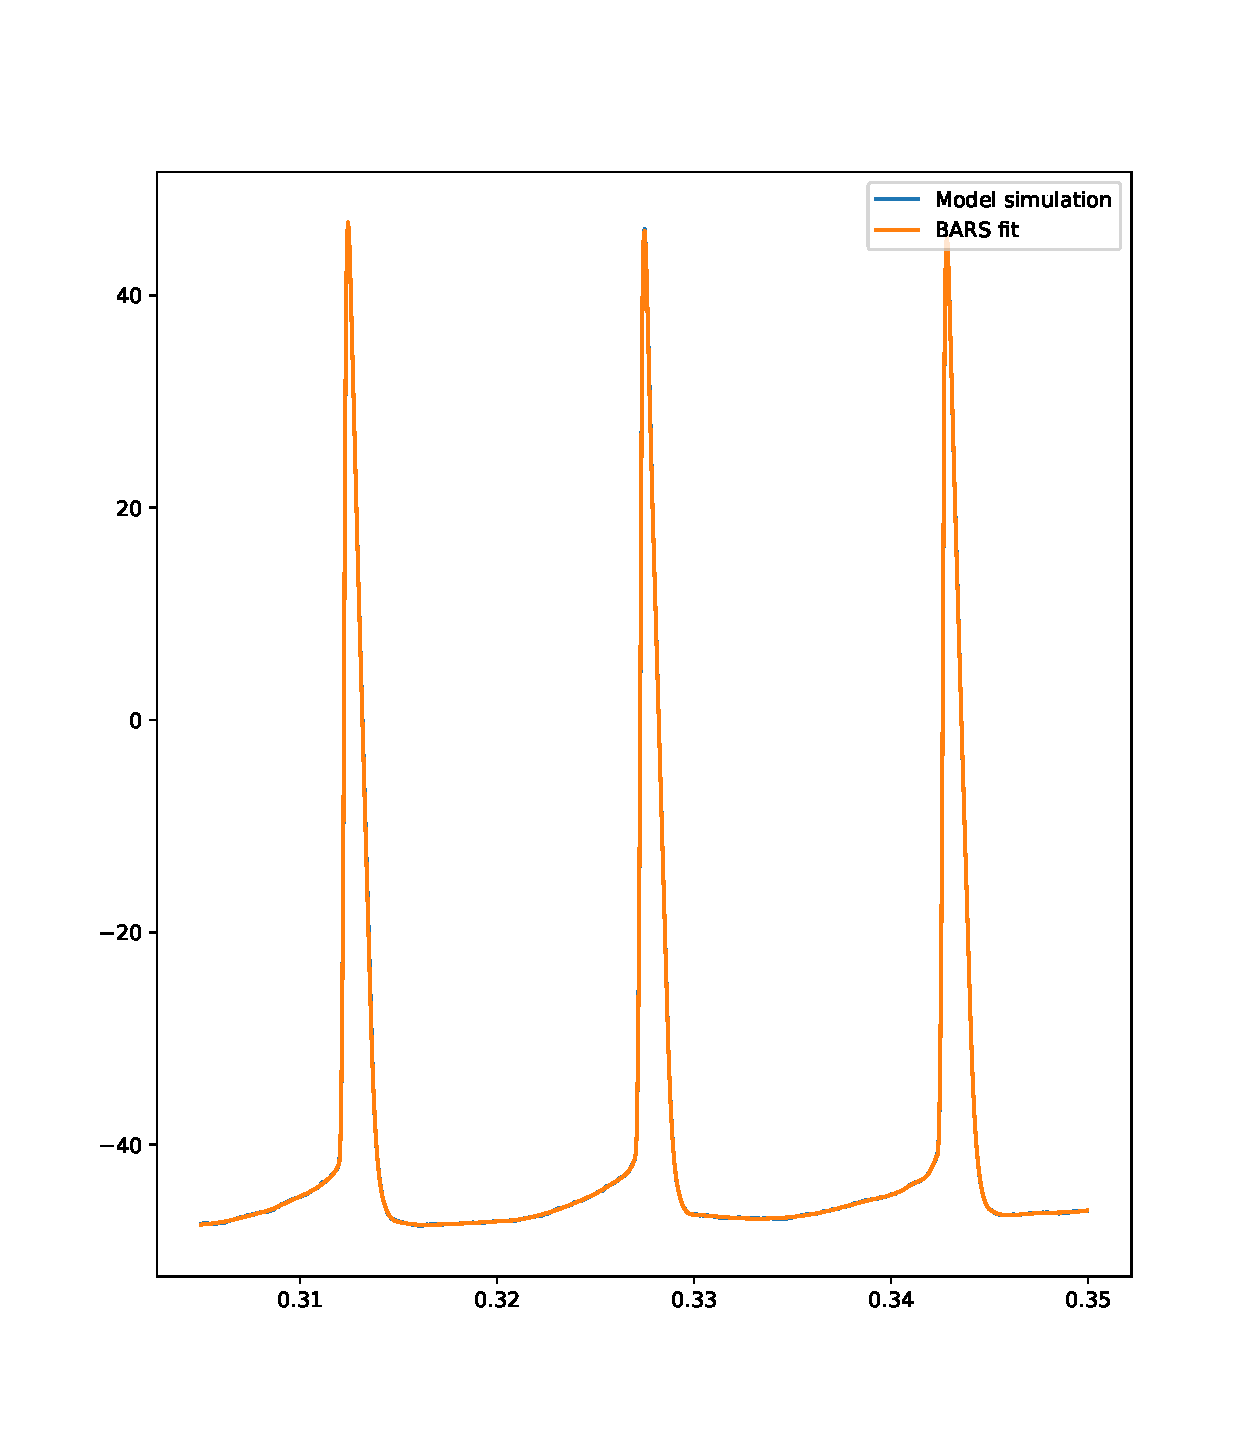
\includegraphics[width=.9\linewidth]{./BARS.pdf}
\end{center}
\end{column}

\begin{column}{0.5\columnwidth}
\begin{center}
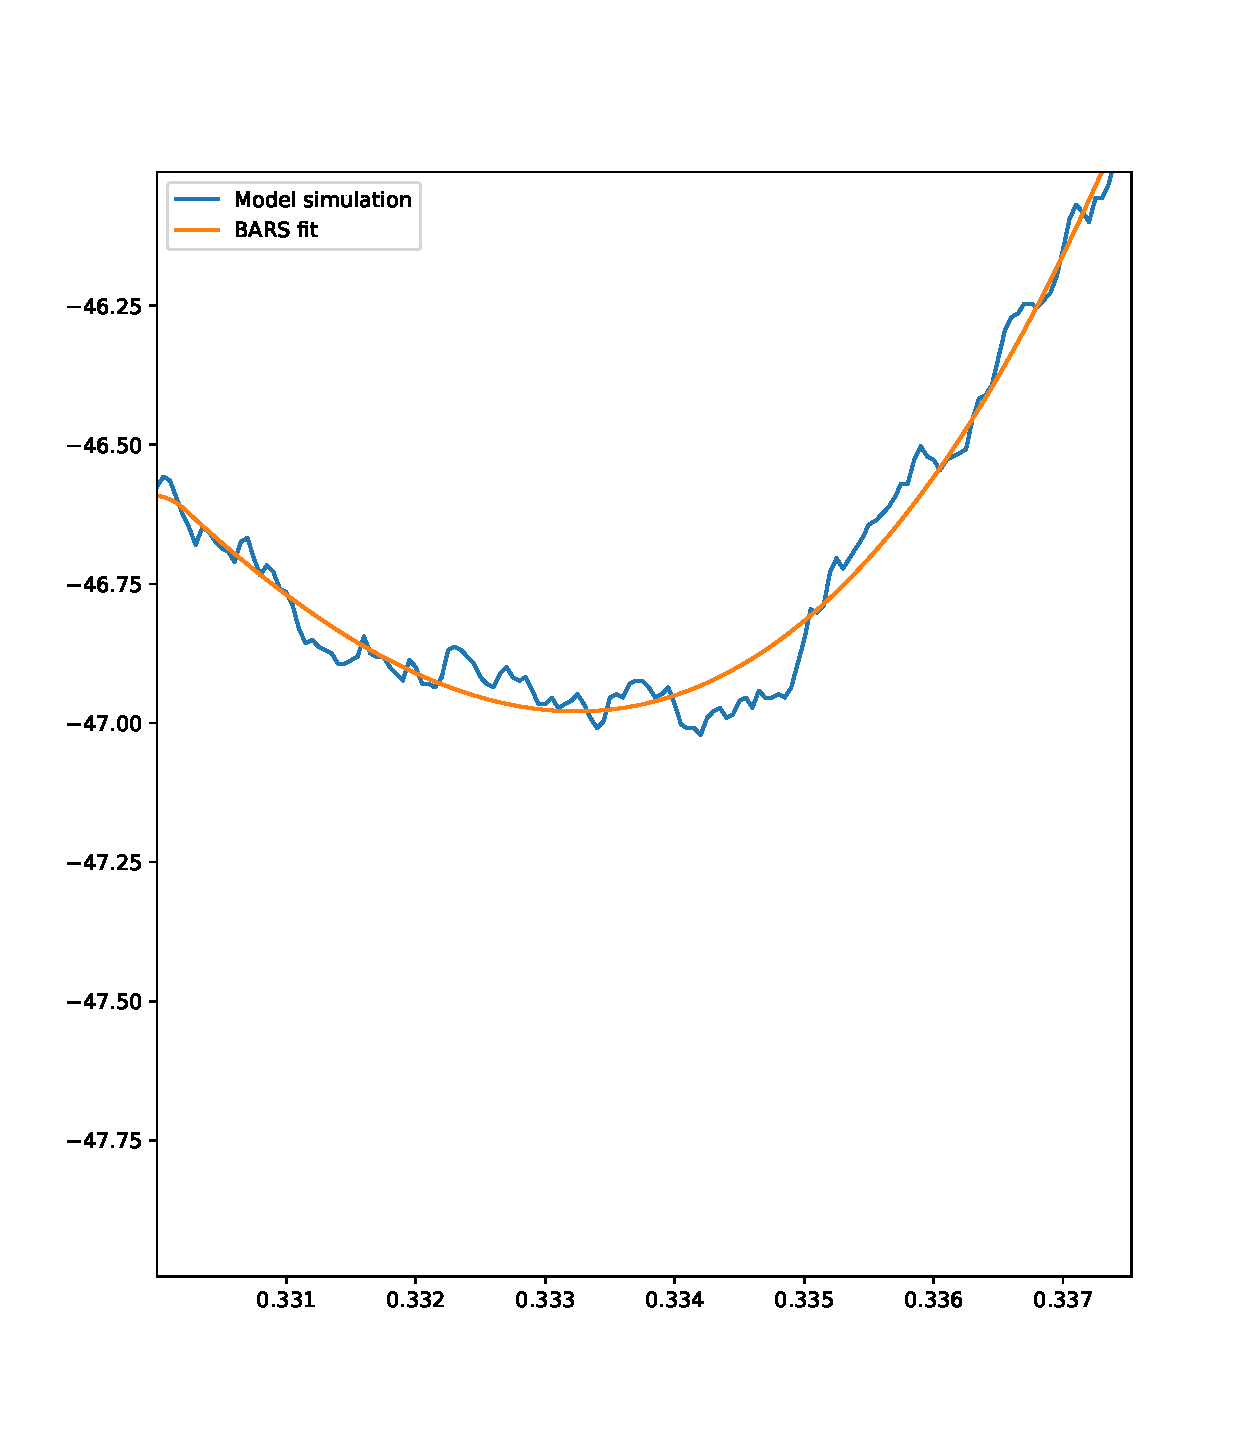
\includegraphics[width=.9\linewidth]{./BARS2.pdf}
\end{center}
\end{column}
\end{columns}
\end{frame}


\begin{frame}[label={sec:org887c574}]{How it works}
\begin{enumerate}
\item Assume a spline model fits the data
\item Find a distribution over spline models, given the data
\item Condition on this distribution with new data, to get posterior estimates
\end{enumerate}
\end{frame}

\section{Step 1}
\label{sec:org2934df8}
\begin{frame}[label={sec:org6a095b3}]{Step 0: problem setup}
\begin{itemize}
\item Take some data \(Y_i = g(x_i) + \varepsilon\)
\begin{itemize}
\item \(\varepsilon\sim\mathcal{N}\{0, \sigma^2\}\)
\item \(\sigma\) unknown
\item \(g\) unknown
\item \(Y_i\) random variables
\item Then, \(Y_i|x_i, \sigma\sim\mathcal{N}\{g(x_i), \sigma^2\}\)
\end{itemize}
\end{itemize}
\vfill
\begin{itemize}
\item Goal: estimate \(g\) from noisy samples \((x_i, Y_i)\)
\end{itemize}
\vfill
This is a very standard problem formulation so far\ldots{}
\end{frame}

\begin{frame}[label={sec:org818d3a3}]{Step 1: spline model}
\begin{itemize}
\item Model latent function \(g\) as being some piecewise-polynomial function \(f\)
\item Tie polynomials together at knot-points \(\xi_i\)
\end{itemize}

\begin{equation}
f(x) = 
    \begin{cases}
        f_1(x)~, \quad x\in[a,\xi_0)\\
	f_2(x)~, \quad x\in[\xi_0, \xi_1)\\
	\dots \\
	f_{k+2}(x)~,\quad x\in[\xi_k, b]
    \end{cases}
\end{equation}

\begin{itemize}
\item \(f_i(x)\) is an \(\mathcal{O}(3)\) polynomial passing through \((\xi_{i-1},g(\xi_{i-1}))\), \((\xi_i, g(\xi_i))\)
\begin{itemize}
\item \ldots{}or allow the polynomials to pass \emph{near} the knot-points, for smoothing splines
\end{itemize}
\end{itemize}
\end{frame}

\begin{frame}[label={sec:org5f97c8a}]{Spline bases}
\begin{itemize}[<+->]
\item Calculating the coefficients for each \(f_i\) is inconvenient
\item Nicer approach:
\begin{itemize}
\item Let \(f(x) = \sum_i \beta_i b_i(x)\)
\item Functions \(b_i\) form a basis for some spline \(f(x)\) with \(k\) knots at \(\{\xi_0, \dots, \xi_k\}\)
\end{itemize}
\item \(b_i\) are found by
\begin{itemize}
\item Specifying knot locations
\item Requiring \(\mathcal{C}^1\) smoothness
\item Assuming linearity outside of data range
\end{itemize}

\item \(b_i\) are called basis splines
\begin{itemize}
\item Our model now becomes \(Y_i | x_i, \beta, \sigma, \xi \sim \mathcal{N}\{\sum_i \beta_i b_i(x_i), \sigma^2\}\)
\end{itemize}
\end{itemize}
\end{frame}

\begin{frame}[label={sec:orgcefff1f}]{Easy approach}
\begin{itemize}[<+->]
\item Choose a nice number of knots \(k\)
\item Choose a uniformly spaced knot-set \(\xi\)
\item Guess \(\sigma\)
\item Find a MLE for \(\beta\)
\end{itemize}

\vfill

Downside: bad choices for any of these parameters will give bad results:

\begin{itemize}[<+->]
\item Too few knots = underparameterised = can't capture shape of data
\item Too many knots = overparameterised = overfit data and capture noise
\item Bad knot positioning = function can't adapt to changing rates
\item How can we infer these from the data?
\end{itemize}
\end{frame}

\section{Step 2}
\label{sec:org1847578}

\begin{frame}[label={sec:org737ea0a}]{Step 2: find a distribution over models}
\begin{itemize}[<+->]
\item Specify a prior belief \(\pi_k(k)\) for the numer of knots we have
\begin{itemize}
\item Eg. discrete uniform on \([k_{min}, k_{max}]\)
\end{itemize}
\item Specify a prior belief \(\pi_\xi(\xi|k)\) on the knot positions \(\xi\), for any given number of knots
\begin{itemize}
\item Eg. uniform on range of data
\end{itemize}
\item Specify a prior belief \(\pi_\sigma(\sigma)\) on the noise level
\item Specify a prior on \(\beta\)
\end{itemize}

Joint probability: \(p(k,\xi,\beta,\sigma,y) = p(y|\beta, \sigma)\pi_\sigma(\sigma)\pi_\beta(\beta|\sigma,\xi,k)\pi_\xi(\xi|k)\pi_k(k)\)

We can evaluate all of this!
\end{frame}

\begin{frame}[label={sec:org55761e3}]{Bayesian approach}
\begin{itemize}
\item We want to know where to put the knots
\item Bayesian approach: find the posterior knot distribution \(p(k, \xi | y)\)
\end{itemize}
\begin{align}
p(k, \xi | y) &= \frac{p(k, \xi, y)}{p(y)}~, \\
p(k, \xi, y) &= \int\int p(k, \xi, \beta, \sigma, y)\mathrm{d}\beta\mathrm{d}\sigma \\
&= \int\int p(y|\beta, \sigma)\pi_\sigma(\sigma)\pi_\beta(\beta|\sigma,\xi,k)\pi_\xi(\xi|k)\pi_k(k)\mathrm{d}\sigma\mathrm{d}\beta
\end{align}
\end{frame}

\begin{frame}[label={sec:org5ea4c32}]{Bayesian approach}
Putting it together, we get

\begin{align}
p(k, \xi | y) &= \frac{\int\int p(y|\beta, \sigma)\pi_\sigma(\sigma)\pi_\beta(\beta|\sigma,\xi,k)\pi_\xi(\xi|k)\pi_k(k)\mathrm{d}\sigma\mathrm{d}\beta}{p(y)} \\
&= \frac{\int\int p(y|\beta, \sigma)\pi_\sigma(\sigma)\pi_\beta(\beta|\sigma,\xi,k)\pi_\xi(\xi|k)\pi_k(k)\mathrm{d}\sigma\mathrm{d}\beta}{\sum_k \int\int\int p(k, \xi, \beta, \sigma, y)\mathrm{d}\xi\mathrm{d}\beta\mathrm{d}\sigma}
\end{align}

\ldots{}which is analytically intractable
\end{frame}

\begin{frame}[label={sec:org92a1841}]{MCMC sampling}
\begin{itemize}
\item Bayesian inference gives posteriors of form
\end{itemize}

\[
\mathrm{posterior} = \frac{\mathrm{likelihood} \times \mathrm{prior}}{\mathrm{Normalising ~constant}}
\]

\begin{itemize}
\item The normalising constant is regularly analytically intractable
\item Markov-chain Monte carlo methods allow us to sample from the posterior distribution anyway
\end{itemize}
\end{frame}

\begin{frame}[label={sec:orgfa42fa2}]{MCMC}
MCMC sets up a Markov chain whose stationary distribution is equal to the posterior distribution:
\begin{itemize}[<+->]
\item Generate a random state from a proposal distribution
\item Accept it with some probability
\item Reject it with some probability
\item On acceptance, change the current state to the accepted state; else, remain at current state
\item Acceptance and rejection probabilities are chosen such that the distribution of accepted states matches that of the prior
\item Doesn't require us to calculate the normalising constant!
\end{itemize}
\end{frame}

\begin{frame}[label={sec:org1f668c7}]{Reversible-jump MCMC}
\begin{itemize}
\item States are the model configuration \((k, \xi)\)
\item These are of many different dimensions
\item To sample from a posterior with varying dimension, we use reversible-jump MCMC
\begin{itemize}
\item Jump up and down in dimension, probabilistically
\item Do so in such a way that the posterior is accurate both within and across dimensions
\end{itemize}
\end{itemize}
\end{frame}

\section{Step 3}
\label{sec:org6c7da0f}
\begin{frame}[label={sec:org49c736d}]{Model inference}
\begin{itemize}
\item Using RJMCMC, we can sample from the posterior \(p(k, \xi | y)\), even though the dimensionality of \(\xi\) is not fixed
\item We can use samples \(k, \xi | y\) to condition on new data \((x^*, y^*)\)
\begin{itemize}
\item \(p(y^* | x^*, x, y) = p(y^*|k, \xi, x^*)p(k, \xi|y)\)
\end{itemize}
\end{itemize}
\vfill
\begin{itemize}
\item We predict new points without ever actually setting up a splines model
\begin{itemize}
\item Find a probability distribution over candidate splines models
\item Weight each spline model's output according to its probability
\end{itemize}
\end{itemize}
\end{frame}


\section{Results}
\label{sec:org688c7bb}
\begin{frame}[label={sec:org4939171}]{My results}
\begin{itemize}
\item Three different MCMC actions can be taken
\begin{itemize}
\item Add a new knot
\item Relocate a knot
\item Delete a knot
\end{itemize}

\item Each action has a proposal probability (how likely are we to take this action?)
\item Each step has an acceptance probability (how likely are we to accept this action?)
\item The BARS paper does a rather bad job of explaining these!
\end{itemize}

In my implementation, probabilities are sometimes coming back negative, making it crash
\end{frame}

\begin{frame}[label={sec:orgf7571f1}]{Results}
\begin{itemize}
\item Results can't be trusted!
\end{itemize}

\begin{center}
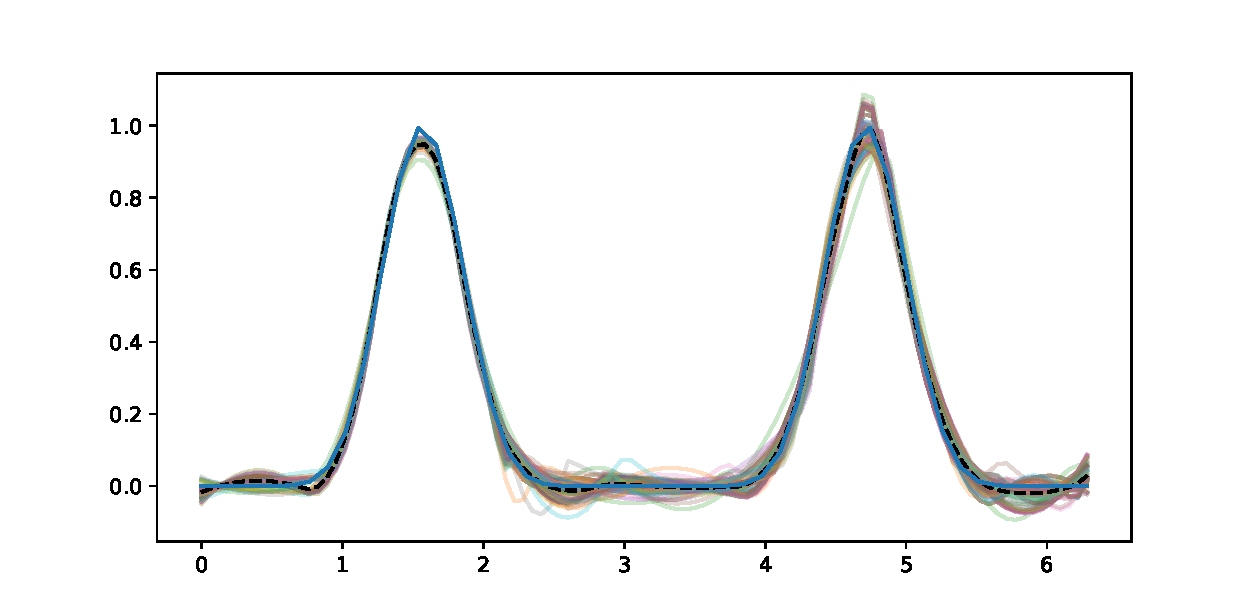
\includegraphics[width=.9\linewidth]{./burnin.pdf}
\end{center}
\end{frame}

\section{BARS GPR}
\label{sec:orgd510f21}
\begin{frame}[label={sec:orgcde83d4}]{BARS and GPR}
\begin{itemize}
\item BARS maintains a distribution over splines
\item GPR maintains a distribution over arbitrarily many functions
\item Both methods refine the distribution with Bayesian methods
\end{itemize}

\vfill

\begin{itemize}
\item BARS probabilistically finds the most informative knot point configuration
\begin{itemize}
\item Finds set of spline-points that tell us the most about the data
\item Sparse GPR probabilistically finds the most informative inducing points distribution
\end{itemize}
\item Tenuous link to optimal experiment design?
\end{itemize}
\end{frame}


\section{Next steps}
\label{sec:org8989dca}
\begin{frame}[label={sec:org8b67076}]{Next steps}
\begin{enumerate}
\item Redraft paper
\item Get BARS to work
\begin{itemize}
\item Useful as it's the most promising method for a conference abstract
\item Either get my implementation working, or adapt C code to my needs
\end{itemize}
\item Fix MSPEs
\begin{itemize}
\item \emph{Should} be quick and easy
\end{itemize}
\item (Re)validate all the models I'm playing with
\item Put results into a conference abstract
\end{enumerate}
\end{frame}
\end{document}
